\section{Optimisation - OpenMP}
Lastly, we optimised the code using OpenMP. For this, we reverted back to code used prior to pthreads. For this, we simply added a line of code above our computationally costly for loop. Before running this code, we run in the command line 'export OMP\_NUM\_THREADS=x', where $x$ can take any positive integer, but for our cases, we limited ourselves to 1 through 8.
\begin{lstlisting}{language=C}
    void compute_quad_forces(vector_t* forces, quadtree_t* tree, particle_t* particles, int N, double theta_max) {
    #pragma omp parallel for
    for(int i = 0; i < N; i++) {
            forces[i] = quad_force(tree, particles[i], theta_max);
    }
}
\end{lstlisting}
From the graph, we can see that OpenMP is more effective than pthreads with its speedups through the number of threads used on both the laptop and the Fredholm server. What we can also see is that Fredholm also gives better results with more threads than the laptop. This could be down to the server having a more stable system to run the computations with more cores.

Again, we didn't manage to get 8 times speed up with 8 threads, since not all the code has been parallelized, but we are closer with OpenMP.

We also attempted to increase performance with the particle updates function. As we tried this however, it seems as though performance actually dropped, so we didn't include this in the final optimised timings.

\begin{figure}[htb]
  \begin{center}
    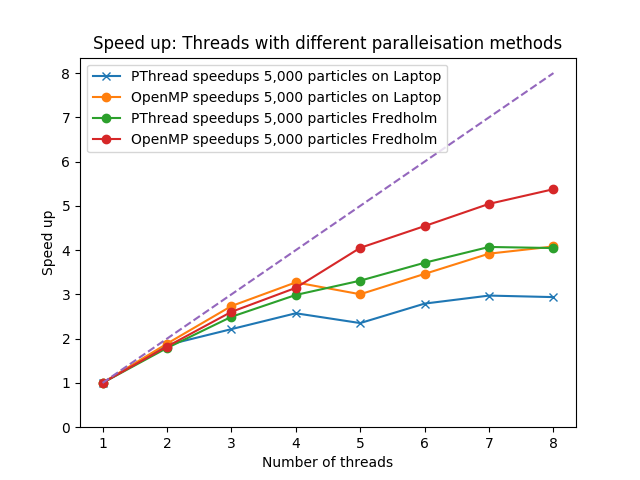
\includegraphics[width=8cm]{../images/openmpVpthread1.png}
    \caption{Speed up graphic: Pthread v OpenMP}
  \end{center}
\end{figure}
\newpage
